\section{Timeliness to Supersafety and Back}\label{sec:forward-reduction}

\subsection{Timeliness $\rightarrow$ Supersafety}

We now construct a supersafe protocol
$\Pi^*$ using a black-box reduction from a safe, live($u$) and timely($v$)
protocol $\Pi$.
Each honest party $P$, executing the $\Pi^*$ protocol, runs a
full node of protocol $\Pi$.
The ledger of party $P$ for protocol $\Pi$ and $\Pi^*$ is denoted as $\Ledger[][P][r]$ and
$\Ledger[*][P][r]$ respectively.
The main idea is that ledger $\Ledger[*][][r]$ is constructed
by filtering through ledger $\Ledger[][][r]$, and only keeping transactions
with recorded round less than or equal to $r - v$.
% When a transaction is written to $P$, it is simply forwarded to the instance of protocol $\Pi$.
The reduction is illustrated
in Figure~\ref{fig:reduction-timeliness-supersafety} and Algorithm~\ref{alg:reduction-timeliness-supersafety}.

\begin{figure}
  \centering
  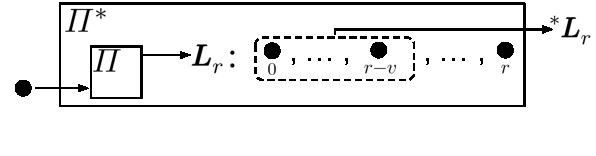
\includegraphics[width=0.7\columnwidth,keepaspectratio]{figures/forward-reduction.pdf}
  \caption{The reduction from Timeliness
    (the $\Pi$ protocol) to Supersafety (the $\Pi^*$ protocol). A transaction is illustrated
    as a black circle and its recorded round is displayed below.
  }
 \label{fig:reduction-timeliness-supersafety}
\end{figure}

When the \rread function is invoked, the temporal ledger of party $P$ is acquired
in Line~\ref{line.reduction-t-s-ledger}.
Then, transactions with recorded round less than or equal to $\now - v$ are
filtered to create $\Ledger[*]$, which is returned in Line~\ref{line.reduction-t-s-filter}.
This introduces a confirmation delay of $v$ additional rounds (see Theorem~\ref{thm:timeliness-to-supersafety}).
When the \wwrite function is invoked with transaction $\tx$, party $P^*$ simply writes $\tx$
to party $P$ in Line~\ref{line.reduction-t-s-write}.

\import{./}{algorithms/algorithm-forward-reduction.tex}

Before proving protocol $\Pi^*$ is supersafe, we present
the following lemma\footnote{
  A variant of this auxiliary lemma was introduced and proven in earlier work~\cite{rollerblade}.
}, which allows us to argue that all
parties in protocol $\Pi$ share a common view of sufficiently old transactions.

%TODO: Add figure for Past Perfect lemma
%TODO: Clean up network activity: as at least one new honest transaction $\tx'$
%      appears in the network at any round $r_3$, where $r_1 < r_3 \leq R - u$.


\begin{lemma}[Past Perfect]\label{lem:past-perfect}
  Consider a safe, live($u$), and timely($v$) temporal ledger protocol
  execution with duration $R$ rounds.
  If for some honest party $P_1$ and some round $r_1$ it holds that
  $(r^*, \tx) \in \Ledger[][P_1][r_1]$, then
  for all honest parties $P_2$ and for all rounds $r_2 \geq r^* + v$
  it holds that $(r^*, \tx) \in \Ledger[][P_2][r_2]$,
  as long as at least one new honest transaction $\tx'$ appears in the
  network at any round $r_3$, where $r_1 < r_3 \leq R - u$.
  \textcolor{red}{Check the upper bound on $r_3$. Should it be $r_2 - u$? Also, do we then need a condition that $v \geq u$?}
\end{lemma}
\begin{proof}
  Consider an execution as in the statement and suppose, towards a contradiction,
  that $(r^*, \tx) = \Ledger[][P_1][r_1][k]$ for some $k \in \mathbb{N}$,
  but $(r^*, \tx) \not\in \Ledger[][P_2][r_2]$
  with $r_2 \geq r^* + v$.
  From safety,
  $\Ledger[][P_2][r_2] \prec \Ledger[][P_1][r_1]$ and
  $|\Ledger[][P_2][r_2]| \leq k < |\Ledger[][P_1][r_1]|$.
  Due to liveness, $(r', \tx') = \Ledger[][P_2][r_3 + u][k']$,
  for some $r', k' \in \mathbb{N}$.
  As $\tx'$ is new, it is not in $\Ledger[][P_1][r_1]$.
  Due to safety, $k' \geq |\Ledger[][P_1][r_1]| > k$, and
  $\Ledger[][P_2][r_3 + u][k] = (r^*, \tx)$.
  Therefore,
  $(r^*, \tx) \in \Ledger[][P_2][r_3 + u][|\Ledger[][P_2][r_2]|{:}]$.
  Since $r^* \leq r_2 - v$, this contradicts the timeliness with parameter $v$.\Qed
\end{proof}

% \atnote{Add: The above lemma holds for already booted clients.}

\begin{theorem}[Timeliness to Supersafety] \label{thm:timeliness-to-supersafety}
  An execution of $\Pi^*$, with duration $R$ rounds, is supersafe
  and live($u + v$), if the execution of
  $\Pi$ is safe, live($u$) and timely$(v)$
  as long as at least one new honest transaction appears in the
  network at each round before $R - u$.
\end{theorem}
\begin{proof}
  Consider any honest parties $P_1,P_2$, any round $r$, and any
  $(r^*, \tx) \in \Ledger[][P_1][r]$, where $r^* \leq r - v$.
  From Lemma~\ref{lem:past-perfect} it holds that
  $(r^*, \tx) \in \Ledger[][P_2][r]$.
  From this and from safety, it follows that
  $\Ledger[*][P_1][r] = [(r^*, \tx) \in \Ledger[][P_1][r]: r^* \leq r - v] \preccurlyeq
  [(r^*, \tx) \in \Ledger[][P_2][r]: r^* \leq r - v] = \Ledger[*][P_2][r]$.
  Inversely, $\Ledger[*][P_2][r] \preccurlyeq \Ledger[*][P_1][r]$.
  Therefore, $\Ledger[*][P_1][r] = \Ledger[*][P_2][r]$.
  Lastly, stickiness follows from the stickiness of $\Pi$.
  Therefore, $\Pi^*$ is supersafe.
  Liveness follows from the liveness of $\Pi$ with an added
  confirmation delay of $v$ rounds.
  \Qed
\end{proof}

Note that a new transaction in every round is required for the purpose of the reduction and is not required for building a supersafe protocol in practice.
We note that the above theorem also applies to late-joining clients.

% \atnote{Add: The above theorem holds for already booted clients.}
